\chapter{Estado da Arte} \label{cap:eda}
%2345678901234567890123456789012345678901234567890123456789012345678901234567890

Preliminarmente... \todo{rewrite all}

Falar aqui o que é ontologia, porque isso é importante e como jogos ou a
industria de entretenimento pode ver isso como util.

\section{Modelo Cognitivo Emocional} \label{cap:eda:mce}

Estudos neurológicos recentes \cite{ledoux1998emotional,damasio2004erro}
mostram a importância das emoções na tomada de decisão. A emoção é definida
como um estado físico do corpo e o sentimento é a percepção desse estado
corporal \cite{damasio2004erro}. Além disso, na psicologia há diferentes
modelos que tentam explicar a afetividade.

\citet{scherer2000tnoe} categorizou esses modelos afetivos em quatro
categorias principais. A primeira categoria, modelos dimensionais, visa
descobrir variáveis que representam eixos das classes emotivas e estabelecem
meios de se mover por esses eixos. Os modelos discretos especificam um
conjunto básico de emoções e especificam regras para que o mecanismo evolua.
Já, a categoria dos baseados em significados se preocupa com as situações
em que o sentimento foi ocasionado e tenta descrever estruturas semânticas dos
mesmos. Por fim, os modelos baseados em componentes entendem que os
sentimentos são aprendidos ao longo do tempo e, sendo assim, estudam o elo
entre os sentimentos e as suas situações. Esse elo é montado de diferentes
formas e varia de pessoa para pessoa.

\begin{figure}[t]
  \centering
    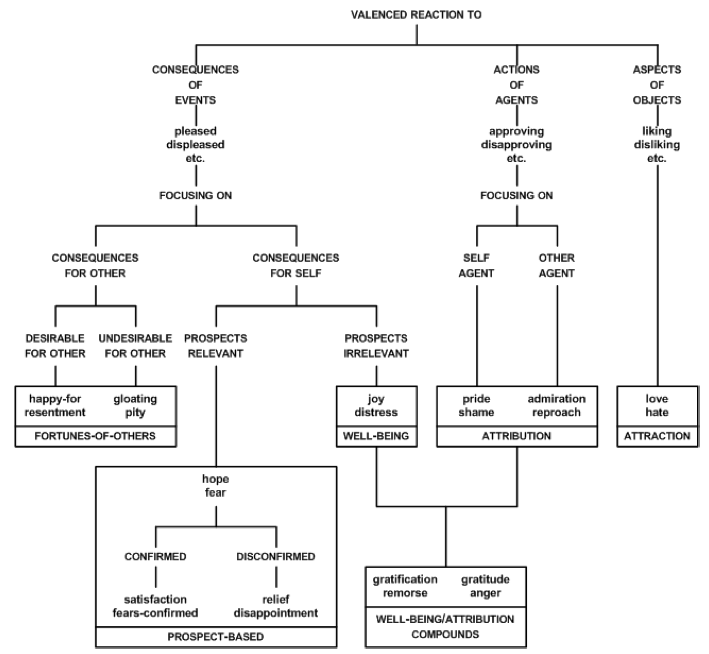
\includegraphics[width=150mm]{figuras/occ.png}
  \caption{Estrutura de emoções \cite{ortony1988cse}.}
  \label{fig:occ_model}
\end{figure}

Um modelo bastante conhecido na Inteligência Artificial foi definido por
\citet{ortony1988cse}. Esse modelo\footnote{A partir daqui o modelo será
referenciado como modelo OCC.} baseado em
significados por descrever as situações de ocorrências de cada uma de suas 22
emoções.  Essas emoções são divididas em formas de se perceber o mundo a sua
volta por consequências (importantes para alguma meta), responsabilidade (pode
se auto julgar) e atração (ou repulsa). Assim sendo, essas maneiras de se
perceber o mundo refletem diferentes jeitos de se analisar as situações que
podem ser relativas aos objetivos, valores morais ou gostos da pessoa.

A Figura~\ref{fig:occ_model} resume esse modelo e mostra as
percepções possíveis de um indivíduo.  Partindo da direita para esquerda, o
ramo mais básico, Aspectos de Objetos, é ativado quando se avalia o gosto de
alguém para algum objeto (inanimado ou não). Por exemplo, alguém gostar de
rosas vermelhas.  No seguinte, Ações de agentes, o julgamento das ações
exercidas por outro indivíduo é realizado baseado nos valores morais da pessoa
que está julgando. Exemplo: reprovar a atitude de um colega que ``colou'' no
teste. Cabe salientar, que julgar ações o modelo permite um grau de
``empatia'' que o autor chamou de ``força cognitiva'' \footnote{Traduzido
literalmente de \emph{Strength of cognitive unit}.}. Dessa forma, é possível,
por exemplo, ficar com orgulho porque uma atleta ganhou uma medalha ou ficar
envergonhado ao descobrir que o vizinho bate no(s) filho(s).

O último ramo da árvore, mais a esquerda na Figura~\ref{fig:occ_model}, é o de consequências de
eventos que representa as coisas que aconteceram (e foram consideradas
importantes), acontecem ou acontecerão (objetivos almejados)\dev{}. Essas
emoções são avaliadas segundo as consequências para o alcance ou impedimento
dos objetivos de uma pessoa. Exemplos desse ramo pode ser a emoção sentida
ao receber uma boa nota em um teste ou, ainda, receber um agradecimento.

Toda a emoção do modelo trabalha com duas intensidades. A intensidade da
emoção que representa o físico e a intensidade do sentimento que representa o
quanto o agente esta percebendo daquela emoção. Dessa forma, um indivíduo só
possui sentimento quando a intensidade da emoção ultrapassa um
determinado\dev{}
limite.  Essa intensidade é obtida por uma função matemática que utiliza
variáveis de dois tipos: local, que influência as emoções do ramo específico;
e global, que influência todas as emoções do modelo.  Um exemplo de variável
local é o desejo, enquanto que um exemplo de variável global pode ser o senso
de realidade.

\citet{bates1994role} afirmou que o comportamento emotivo de um personagem é
um papel importante para ser ter a ilusão de vida. Esse trabalho foi um dos
primeiros à utilizar o modelo descrito visando melhorar a credibilidade de
seus atores ligando cada uma das emoções com um determinado tipo de
comportamento. Por exemplo, um agente liga o medo a um comportamento agressivo
enquanto outro liga essa mesma emoção com um comportamento retraído.

Com a finalidade de demostrar que as emoções melhoraram a credibilidade dos
atores, \citet{zhang2009emotional} desenvolveram uma aplicação. Nesse
trabalho, os sentimentos afetam a forma que o planejamento das ações é
realizado. \citet{neto2010construction} visaram entender o impacto da emoção
na tomada de decisão. Assim, eles fizeram com que agentes pudessem
``esquecer'' determinadas crenças quando o estado emocional fosse diferente
daquele guardado anteriormente. Essa característica torna o planejamento e as
atitudes dos personagens virtuais mais realistas.

O objetivo de \citet{bick2003relational} com o projeto \emph{Relational
Agents} é possibilitar aos usuários a criação de um relacionamento social e
emocional com longa duração.  Em \citet{bickmore2009virtual}, a confiança no
agente tornou possível discutir tarefas mais importantes como melhoria da saúde
ou até a compra de uma casa. Da mesma forma, o projeto
AIDA\footnote{Mais detalhes, ver \url{http://senseable.mit.edu/aida}.} (do
inglês \emph{Affective Intelligent Driving Agent}) pode ser entendido como
enquadrado na área de Interface Homem Computador, pois o interesse é entender o
estado afetivo da pessoa dirigindo. Além disso, o agente pode tentar sugerir
ao usuário mudanças em suas rotas baseado na rotina aprendida anteriormente.

Um dos trabalhos mais conhecidos utilizando o modelo OCC é, sem dúvida, o de
\citet{kshirsagar2002multilayer}. Ele utilizou as emoções levantadas no modelo
em conjunto com um modelo de personalidade baseado na psicologia que leva em
consideração 5 fatores. O primeiro fator, extroversão, é descrito como a
preferência para o comportamento em situações sociais. O segundo,
agradabilidade, é a interação com outras pessoas. Outro fator é a
conscientização que é a organização e persistência das metas. A tendência de
pensamentos negativos é o chamado fator neurótico. O último é o que descreve
se a pessoa tem interesse em cultura ou é ``cabeça aberta''.\todo{falar mais?}

\section{Ontologias Emocionais} \label{cap:eda:oe}

Ontologias emocionais são ontologias que visam descrever as emoções ou
aspectos afetivos de um indivíduo se baseando em estudos da psicologia.
...

Em \citet{benta2007ontology} foi feita a construção de uma ontologia escrita
em \emph{OWL}. Nesse trabalho as emoções são divididas em primárias e
secundárias, e as secundárias se originam a partir das primárias. As emoções
primárias ou básicas, não cognitivas, são: brabo, desgosto, feliz, medo,
neutro, surpreso e triste. As emoções secundárias, cognitivas, descritas são
ao todo 4. O interessante aqui é que essas 4 emoções são inferidas a partir
de propriedades de objeto. Além disso, há o conceito de emoção ativa que é a
emoção predominante naquele momento. O valor da emoção é calculado da seguinte
forma, a sensibilidade (predisposição a emoção que varia de 0 à 1)
multiplicado pela intensidade da emoção. A emoção predominante é o maior valor
entre as emoções.

Não tendo nenhuma informação de uma teoria de emoções específicas modeladas em
sua ontologia, \citet{wks2008towards} criou uma ontologia de alto nível se
aproveitando de outra ontologia de alto nível e de uma de analise léxica. O
principal conceito da ontologia pode ser pensado como o de sensores que são
objetos físicos que recebem informações do ambiente e as ``transportam'' para
o mundo mental. Sendo assim, é possível reconhecer a percepção recebida
utilizando a memória e descrever a nova situação. Por não conter dados
específicos de uma teoria de emoção, a ontologia gerada é de um nível mais
alto. Todavia, o presente trabalho não tem esse objetivo\dev{}.

No modelo definido por \citet{ortony1988cse} entre emoções primárias e
secundárias não existe porque se pressupõe que toda emoção exige um certo
nível de cognição. Não existe um limite no que pode ou não ser percebido em
quantidade de emoções, mas se pode pensar que os valores que influencia dois
atributos opostos são os mesmos e, por isso, eles não serão sentidos ao mesmo
tempo. Além disso, o modelo utilizou a diferenciação entre emoção e sentimento
proposta por \citet{damasio2004erro}. Ele diz que sentimento é a percepção da
emoção, enquanto a emoção não seria percebida.

\citet{springerlink:10.1007/978-3-642-01639-448} desenvolveu um motor de
emoções que utiliza um modelo de mistura de emoções em conjunto com o modelo
OCC. O trabalho deles dividiu o modelo em camadas, nas quais cada camada tem
uma responsabilidade distinta e que visa complementar a anterior. A
camada de classificação visa determinar que categoria ou ramo será afetado. A
seguinte de quantificação determina a intensidade da emoção. A de interação
analisa os efeitos nas categorias emocionais do personagem. A próxima mapeia
as 22 emoções do modelo para pelo menos uma expressão e a última camada é a
responsável por realizar a expressão propriamente dita no ator.

Esse trabalho ainda utilizou um modelo dimensional para misturar as emoções
primárias. Assim, as emoções secundárias podem ser descobertas a partir dos
eixos do nível dos eixos afetados. O trabalho mostra somente 10 emoções do
ramo de consequência de eventos, com exceção das emoções de esperança (Hope) e
medo não confirmado (Fear). As emoções do modelo OCC são consideradas as
emoções primárias e como secundárias estão as emoções construídas a partir da
mistura de outras emoções. Como dito anteriormente, estaria incorreto fazer
essa diferenciação no modelo sendo proposto porque ela não é realizada no
modelo OCC original.

\todo{to na duvida se isso fica...}\citet{adam2009alfototoe} formalizaram o modelo OCC de maneira lógica. A
formalização construída possui algumas limitações, por exemplo em nenhum ponto
do trabalho é mencionado o ramo de objetos e no ramo de ações é desconsiderado
a empatia (ou força de unidade cognitiva) com outros indivíduos. Além disso,
no ramo de eventos a probabilidade é medida de forma comparativa, isto é, o
evento A é mais que provável que o evento B. Fora isso, para a formalização
ser feita é necessário estabelecer uma ordem temporal das ações sendo
realizadas. Entretanto, o autor propõem uma diferenciação entre ação e evento.
O primeiro é causado intencionalmente pelo agente, enquanto o segundo o agente
não tem controle da ação. Por exemplo, o ato de espirrar seria um evento.

Um modelo genérico que representa o ambiente e eventos que estão envolta de um
personagem, sua personalidade e preferencias foi feito por
\citet{lera2009semantic}\todo{falar mais}. Nesse trabalho o foco eram emoções
que podem ser representadas no rosto. Assim, a identificação do contexto
através de eventos e do retorno afetivo. Além disso, as expressões faciais são
modificadas dependendo dos eventos do ambiente e, também, da personalidade,
metas e preferências dos atores virtuais.


\section{Ontologias de Humanos Virtuais} \label{cap:eda:odhv}

Uma ontologia descrevendo humanos virtuais tem inúmeras utilidades tanto em
pesquisa quanto na indústria. A mesma pode servir tanto para descrever a forma
física quanto a forma mental ou, melhor, comportamental. Essas duas
possibilidades podem ser de grande valia, na indústria se esta interessado em
tentar reaproveitar o máximo possível desses recursos. Por exemplo, obter um
personagem de um banco de dados a partir da descrição ``mulher de cabelo
preto''. Da mesma forma, é possível focar no aspecto comportamental do humano
virtual descrevendo determinados comportamentos ou planos de ações de atores.
No trabalho de \citet{Gutierrez:2007:OVH:1229160.1229164} a excelentes
exemplos do uso de uma ontologia de humano virtual.

\begin{figure}[t]
  \centering
    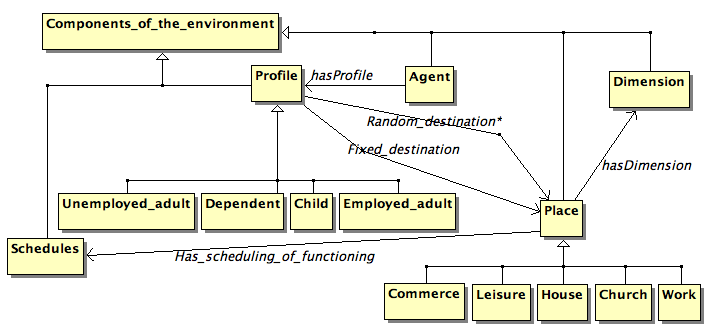
\includegraphics[width=150mm]{figuras/UEMontology.png}
  \caption{Modelo de ambiente urbano \cite{paiva2005ontology}.}
  \label{fig:UEM}
\end{figure}

A primeira ontologia a ser abordada descreve o comportamento habitual de
atores em uma determinada cidade virtual. Essa ontologia, mostrada na
Figura~\ref{fig:UEM}\footnote{As relações de generalização possuem a mesma
semântica que na UML, as relações direcionais são relações binárias entre as
instâncias das classes.}, foi apresentada durante a introdução do \emph{Urban
Environment Model} no trabalho de \citet{paiva2005ontology}. Nesta há 5
conceitos principais, o primeiro conceito \emph{Agent} se relaciona com o
conceito \emph{Profile} para determinar o tipo de agente. O perfil do agente
pode variar entre \emph{Unemployed Adult}, \emph{Employed Adult}, \emph{Child}
e \emph{Dependent}. Os tipos \emph{Child} e \emph{Employed Adult} possuem
destinos fixos em determinados momentos do dia e, depois, destinos randômicos.
\emph{Unemployed Adult} só possui destinos randômicos e \emph{Dependent}
necessita de um adulto para se mover.

Assim, o perfil do agente permite definir locais usuais (fixos) e eventuais
(randômicos). Esses locais são definidos pelo conceito \emph{Place} que contêm
uma descrição de sua capacidade (quantidade máxima de atores), dimensão
(acessível por relação) e horário de funcionamento (acessível por relação). O
conceito de \emph{Dimension} guarda possui a posição dos eixos X e Y, altura e
largura. Finalmente, o último \emph{Schedules} possui o horário de abertura e
fechamento, intervalo de entrada e tempo médio de permanência. Esse modelo é
muito simplista porque o foco é possibilitar que uma maior quantidade de
agentes sejam carregados. Além disso, todos os agentes não possuem uma decisão
ou desejo sobre suas próprias metas. Essa decisão é feita pelo ambiente que
impele o ator para ir em determinado lugar através do seu conhecimento do
perfil dos atores.

Este trabalho pode ser pensado como a tentativa de descrever a mentalidade dos
personagens através da descrição dos atores em um ambiente urbano em sua vida
normal. O foco da ontologia seguinte é o humano virtual propriamente dito.
Assim, as informações gerais do personagem, como, por exemplo, raça, cor e
outros são armazenadas na ontologia descrita visando uma descrição completa e
reusável. A Figura~\ref{fig:OVH} apresenta os principais conceitos da
ontologia desenvolvida por \citet{Gutierrez:2007:OVH:1229160.1229164}.

O conceito principal definido na ontologia é o \emph{Virtual Human}. O modelo
pode ser utilizado para representar pessoas virtuais ou reais. Humanos
virtuais podem serem descritos por \emph{Structural Descriptors} e
\emph{Morphological Descriptors}. Neste último são guardados os dados gerais
do personagem, por exemplo idade, sexo, altura, peso e etc. No outro conceito,
\emph{Structural Descriptors} é uma abstração que define os pontos de entrada
para uma variedade de descritores que descrevem a organização do humano
virtual. No modelo o foco foi organização por esqueleto e se baseando na
especificação H-Anim\footnote{É uma especificação que descreve quantidade,
posição e rotação dos ossos para tentar padronizar os modelos.
Veja \url{http://www.h-anim.org/}.} e como pode ser visto é possível guardar
informações de geometria, textura e outras informações.

\begin{figure}[t]
  \centering
    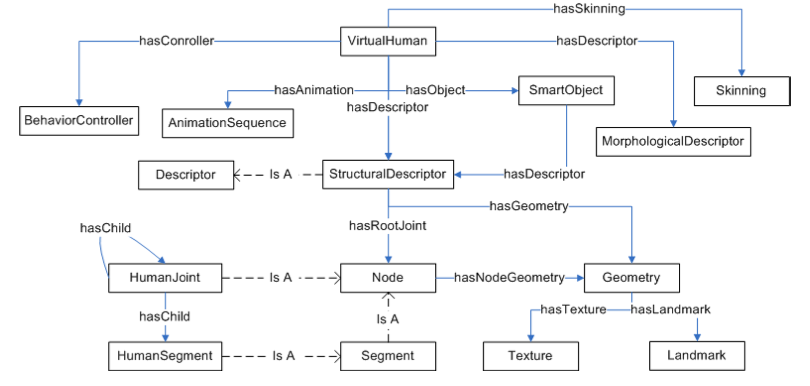
\includegraphics[width=150mm]{figuras/gutierrezVH.png}
  \caption{Ontologia de Humano Virtual \cite{Gutierrez:2007:OVH:1229160.1229164}.}
  \label{fig:OVH}
\end{figure}

Assim, o corpo humano consiste de um número de \emph{Segment} (por exemplo,
pé, mão e etc) que são conectados por \emph{Node}. Cada \emph{Node} pode
conter outros e, também, um \emph{Segment}. Além disso, o humano virtual pode
ser animado de duas formas. A primeira é através de uma animação sequencial
pre-gravada representada pelo conceito \emph{Animation Sequence} e a segunda é
utilizando o conceito de \emph{Behavioral Controller}. Esse último pode ser
utilizado para embutir com um comportamento mais autônomo. Por fim, o conceito
de \emph{Smart Object} representa todos os objetos que podem ser manipulados por
um humano virtual.

%2345678901234567890123456789012345678901234567890123456789012345678901234567890
